
\Programme{Higher Diploma in Science in Computer Science (Online)}
\def\PROGRAMME{HDip in Computer Science}

\vspace{-50pt}

\vspace{0cm}

The ONLINE {\bfseries Higher Diploma in Science in Computer Science} is an accelerated 24-month ICT Conversion Course focused on full stack oriented development. It is designed to allow honours graduates from non-computing disciplines to acquire the industry-relevant ICT and software development skills, expertise and practical experience required to become suitable candidates for employment in the ICT domain in general and in software development in particular.


\vspace{9pt}

\centerline{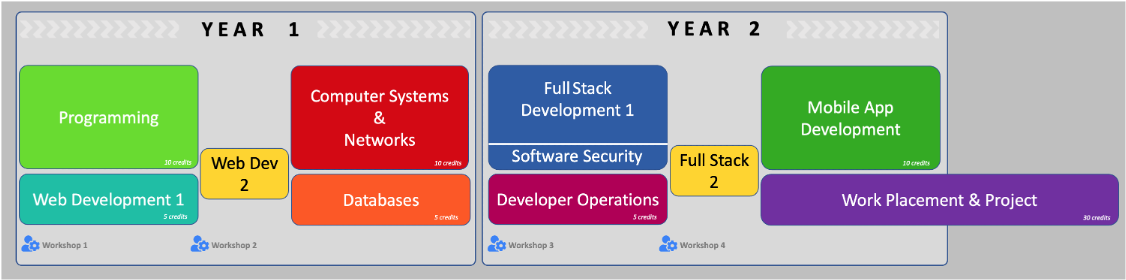
\includegraphics[width=19cm]{../common_images/orig/hdip_struct}}

\vspace{9pt}

As an accelerated course, there is an average time commitment of 16 hours per week required. Students with less ICT experience may need to factor in more time. The course is delivered using our award-winning online delivery platform---TutorStack. Pioneered on this programme with industry, we follow an ``Agile Semester'' approach, typically consisting of 4, three-week sprints followed by 1-week breaks for retrospective, after each sprint.

\vspace{12pt}
\mbox{}\hfill
\begin{minipage}{.32\textwidth}
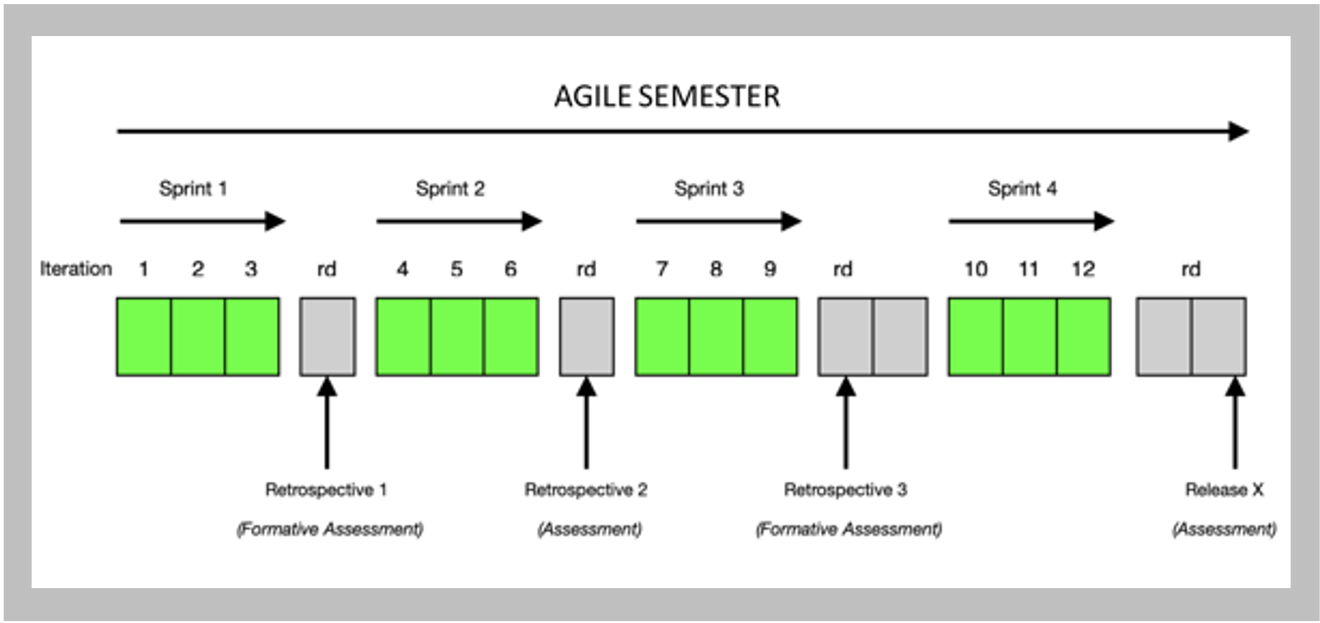
\includegraphics[width=\textwidth]{../common_images/orig/hdip_agile}
\end{minipage}\hfill
\begin{minipage}{.56\textwidth}
In addition there is a six lesson on-demand module each summer. Online delivery over the two years is supplemented by four onsite workshops to further enhance and deepen the learning experience, and learning community. Although not mandatory, these should be deemed essential. While all taught modules are delivered within two years, Work Project \& Placement runs into the following year so as not to over burden students.

\vspace{9pt}
For a more in depth preview of the course content and structure, please watch this 
\href{https://youtu.be/opRwmuwbf0I}{video}.

\vspace{9pt}
Try out a sample of the course \href{https://wit-hdip-comp-sci.github.io/}{here}.

\vspace{9pt}
\href{https:/www.wit.ie/courses/hdip-computer-science-parttime}{Find out more here}.

\vspace{-12pt}
\end{minipage}\hfill
\clearpage

%\projectstoc

%\clearpage
%\begin{center}
%\typesetPhotoTOC{6}{3.25cm}
%\end{center}

%\clearpage

%\typesetPhotoTOCGROUPS{6}{3cm}

%: projects

\projectsBegin


\input{../student_content/Leanne_Ahern_33484_content.tex}

\begingroup\globaldefs=1\relax

%: SID
\pgfkeyssetvalue{/students/Ludmila_Bulat_41BE2/SID}{[SID]}


%: Key
\def\Key{Ludmila_Bulat_41BE2}
\pgfkeyssetvalue{/students/Ludmila_Bulat_41BE2/Key}{Ludmila_Bulat_41BE2}

%: Name
\pgfkeyssetvalue{/students/Ludmila_Bulat_41BE2/Name}
{Ludmila Bulat}
\pgfkeyssetvalue{/students/Ludmila_Bulat_41BE2/SortName}
{Bulat, Ludmila}

%: Programme
\pgfkeyssetvalue{/students/Ludmila_Bulat_41BE2/Programme}
{Higher Diploma in Science in Computer Science}

%: Photo
\pgfkeyssetvalue{/students/Ludmila_Bulat_41BE2/Photo}
{Ludmila_Bulat_41BE2}
\pgfkeyssetvalue{/students/Ludmila_Bulat_41BE2/HasPhoto}
{True}

%: Poster
\pgfkeyssetvalue{/students/Ludmila_Bulat_41BE2/Poster}
{Ludmila_Bulat_41BE2}
\pgfkeyssetvalue{/students/Ludmila_Bulat_41BE2/HasPoster}
{True}
\pgfkeyssetvalue{/students/Ludmila_Bulat_41BE2/PosterWidth}
{3508}
\pgfkeyssetvalue{/students/Ludmila_Bulat_41BE2/PosterHeight}
{2480}
\pgfkeyssetvalue{/students/Ludmila_Bulat_41BE2/PosterOrientation}
{landscape}
\pgfkeyssetvalue{/students/Ludmila_Bulat_41BE2/PosterScale}
{0.9901612903225806}

%: QR
\pgfkeyssetvalue{/students/Ludmila_Bulat_41BE2/QR}
{SD}
\pgfkeyssetvalue{/students/Ludmila_Bulat_41BE2/HasQR}
{True}

%: CommercialTitle
\pgfkeyssetvalue{/students/Ludmila_Bulat_41BE2/CommercialTitle}
{ScanIQ}

%: AcademicTitle
\pgfkeyssetvalue{/students/Ludmila_Bulat_41BE2/AcademicTitle}
{Scaniq: A Mobile Application for Ingredient Analysis Using Barcode Scanning and Food Data APIs}

%: Summary
\pgfkeyssetvalue{/students/Ludmila_Bulat_41BE2/Summary}
{ScanIQ is a mobile application that helps users better understand food products by scanning barcodes and analysing ingredient data. The app integrates the OpenFoodFacts API to retrieve product information and applies a custom scoring system based on nutritional values such as sugar, salt, additives, and fibre. Users receive a simple colour-coded score and clear explanations, along with healthier product recommendations. The application also includes features such as scan history and favourites, focusing on usability, transparency, and informed decision-making.}

%: Technologies 
\pgfkeyssetvalue{/students/Ludmila_Bulat_41BE2/Technologies}
{React Native, Expo, TypeScript, OpenFoodFacts API, AsyncStorage, Expo Camera}

%: ProjectURL
\pgfkeyssetvalue{/students/Ludmila_Bulat_41BE2/ProjectURL}
{https://scaniq-final-project.vercel.app/}

%: SupervisorLabel
\pgfkeyssetvalue{/students/Ludmila_Bulat_41BE2/SupervisorLabel}
{Project Supervisor}

%: SupervisorTitle
\pgfkeyssetvalue{/students/Ludmila_Bulat_41BE2/SupervisorTitle}
{}

%: Supervisor
\pgfkeyssetvalue{/students/Ludmila_Bulat_41BE2/Supervisor}
{Dave Drohan}

%: Room
\pgfkeyssetvalue{/students/Ludmila_Bulat_41BE2/Room}
{TL2.38}

%: Number
\pgfkeyssetvalue{/students/Ludmila_Bulat_41BE2/Number}
{73}

%: ProjectAreas
\pgfkeyssetvalue{/students/Ludmila_Bulat_41BE2/ProjectAreas}
{AI ML Development,Software Development Core,Software Development Front End,Software Development Mobile Hybrid,Personal Independent Project}
\pgfkeyssetvalue{/students/Ludmila_Bulat_41BE2/ProjectAreasTeX}
{\pgfkeysvalueof{/area/AI ML Development/Name}, \pgfkeysvalueof{/area/Personal Independent Project/Name}, Software Development: (Core / Front End / Mobile Hybrid)}
\pgfkeyssetvalue{/students/Ludmila_Bulat_41BE2/ProjectAreasTeX2}
{\pgfkeysvalueof{/area/AI ML Development/Name}, \pgfkeysvalueof{/area/Personal Independent Project/Name}, Software Development: (Core / Front End / Mobile Hybrid)}

\endgroup

\DefaultLayout

\input{../student_content/Nigel_Byrne_2BD13_content.tex}

\begingroup\globaldefs=1\relax

%: SID
\pgfkeyssetvalue{/students/Vincent_Byrne_15519/SID}{[SID]}


%: Key
\def\Key{Vincent_Byrne_15519}
\pgfkeyssetvalue{/students/Vincent_Byrne_15519/Key}{Vincent_Byrne_15519}

%: Name
\pgfkeyssetvalue{/students/Vincent_Byrne_15519/Name}
{Vincent Byrne}
\pgfkeyssetvalue{/students/Vincent_Byrne_15519/SortName}
{Byrne, Vincent}

%: Programme
\pgfkeyssetvalue{/students/Vincent_Byrne_15519/Programme}
{Higher Diploma in Science in Computer Science}

%: Photo
\pgfkeyssetvalue{/students/Vincent_Byrne_15519/Photo}
{Vincent_Byrne_15519}
\pgfkeyssetvalue{/students/Vincent_Byrne_15519/HasPhoto}
{True}

%: Poster
\pgfkeyssetvalue{/students/Vincent_Byrne_15519/Poster}
{Vincent_Byrne_15519}
\pgfkeyssetvalue{/students/Vincent_Byrne_15519/HasPoster}
{True}
\pgfkeyssetvalue{/students/Vincent_Byrne_15519/PosterWidth}
{1346}
\pgfkeyssetvalue{/students/Vincent_Byrne_15519/PosterHeight}
{992}
\pgfkeyssetvalue{/students/Vincent_Byrne_15519/PosterOrientation}
{landscape}
\pgfkeyssetvalue{/students/Vincent_Byrne_15519/PosterScale}
{0.949798387096774}

%: QR
\pgfkeyssetvalue{/students/Vincent_Byrne_15519/QR}
{SD}
\pgfkeyssetvalue{/students/Vincent_Byrne_15519/HasQR}
{True}

%: CommercialTitle
\pgfkeyssetvalue{/students/Vincent_Byrne_15519/CommercialTitle}
{APAVS}

%: AcademicTitle
\pgfkeyssetvalue{/students/Vincent_Byrne_15519/AcademicTitle}
{Automated Pipeline and Visualisation System for Tool Load Port Data}

%: Summary
\pgfkeyssetvalue{/students/Vincent_Byrne_15519/Summary}
{APAVS automates the monitoring of load port qualification data across a fleet of semiconductor manufacturing tools. Currently, technicians manually export log files, run Excel macros, and visually inspect qualification plots for individual tools with no fleet-wide visibility. APAVS replaces this workflow with a PowerShell extraction pipeline that retrieves data directly from tool hard drives, parses raw sensor logs, and calculates slot-level offsets against taught reference positions. Results are stored in a SQL Server database and visualised through a Power BI.}

%: Technologies 
\pgfkeyssetvalue{/students/Vincent_Byrne_15519/Technologies}
{PowerShell, SQL Server, Power BI}

%: ProjectURL
\pgfkeyssetvalue{/students/Vincent_Byrne_15519/ProjectURL}
{https://bit.ly/4rJabZx}

%: SupervisorLabel
\pgfkeyssetvalue{/students/Vincent_Byrne_15519/SupervisorLabel}
{Project Supervisor}

%: SupervisorTitle
\pgfkeyssetvalue{/students/Vincent_Byrne_15519/SupervisorTitle}
{}

%: Supervisor
\pgfkeyssetvalue{/students/Vincent_Byrne_15519/Supervisor}
{Sonya Hogan}

%: Room
\pgfkeyssetvalue{/students/Vincent_Byrne_15519/Room}
{Not Presenting}

%: Number
\pgfkeyssetvalue{/students/Vincent_Byrne_15519/Number}
{75}

%: ProjectAreas
\pgfkeyssetvalue{/students/Vincent_Byrne_15519/ProjectAreas}
{Automotive and Automation,Database and Analytics,Work Based Project}
\pgfkeyssetvalue{/students/Vincent_Byrne_15519/ProjectAreasTeX}
{\pgfkeysvalueof{/area/Automotive and Automation/Name}, \pgfkeysvalueof{/area/Database and Analytics/Name}, \pgfkeysvalueof{/area/Work Based Project/Name}}
\pgfkeyssetvalue{/students/Vincent_Byrne_15519/ProjectAreasTeX2}
{\pgfkeysvalueof{/area/Automotive and Automation/Name}, \pgfkeysvalueof{/area/Database and Analytics/Name}, \pgfkeysvalueof{/area/Work Based Project/Name}}

\endgroup

\DefaultLayout

\input{../student_content/Peter_Chuk_1049E_content.tex}
\input{../student_content/Aidan_Clancy_92AB6_content.tex}
\input{../student_content/Shane_Crowley_E9668_content.tex}
\input{../student_content/Daniel_Cullen_9BC37_content.tex}
\input{../student_content/Eoin_Geoghegan_98F46_content.tex}

\begingroup\globaldefs=1\relax

%: SID
\pgfkeyssetvalue{/students/Wolfgang_Helnwein_16881/SID}{[SID]}


%: Key
\def\Key{Wolfgang_Helnwein_16881}
\pgfkeyssetvalue{/students/Wolfgang_Helnwein_16881/Key}{Wolfgang_Helnwein_16881}

%: Name
\pgfkeyssetvalue{/students/Wolfgang_Helnwein_16881/Name}
{Wolfgang Helnwein}
\pgfkeyssetvalue{/students/Wolfgang_Helnwein_16881/SortName}
{Helnwein, Wolfgang}

%: Programme
\pgfkeyssetvalue{/students/Wolfgang_Helnwein_16881/Programme}
{Higher Diploma in Science in Computer Science}

%: Photo
\pgfkeyssetvalue{/students/Wolfgang_Helnwein_16881/Photo}
{Wolfgang_Helnwein_16881}
\pgfkeyssetvalue{/students/Wolfgang_Helnwein_16881/HasPhoto}
{True}

%: Poster
\pgfkeyssetvalue{/students/Wolfgang_Helnwein_16881/Poster}
{Wolfgang_Helnwein_16881}
\pgfkeyssetvalue{/students/Wolfgang_Helnwein_16881/HasPoster}
{True}
\pgfkeyssetvalue{/students/Wolfgang_Helnwein_16881/PosterWidth}
{3508}
\pgfkeyssetvalue{/students/Wolfgang_Helnwein_16881/PosterHeight}
{2480}
\pgfkeyssetvalue{/students/Wolfgang_Helnwein_16881/PosterOrientation}
{landscape}
\pgfkeyssetvalue{/students/Wolfgang_Helnwein_16881/PosterScale}
{0.9901612903225806}

%: QR
\pgfkeyssetvalue{/students/Wolfgang_Helnwein_16881/QR}
{SD}
\pgfkeyssetvalue{/students/Wolfgang_Helnwein_16881/HasQR}
{True}

%: CommercialTitle
\pgfkeyssetvalue{/students/Wolfgang_Helnwein_16881/CommercialTitle}
{There's No Place Like Home}

%: AcademicTitle
\pgfkeyssetvalue{/students/Wolfgang_Helnwein_16881/AcademicTitle}
{Design and Implementation of a Segmented, Privacy-Centric Homelab Using Open-Source Platforms}

%: Summary
\pgfkeyssetvalue{/students/Wolfgang_Helnwein_16881/Summary}
{'There's No Place Like Home' shows how a typical home network can become a secure, scalable, privacy-focused homelab using open-source tools. It employs VLAN-based segmentation, a custom OPNsense router, a managed switch, and Proxmox for self-hosting to enable network isolation and flexible service deployment. Focused on hands-on learning, the project develops systems administration and architecture skills through iterative, experiential practice. Favouring locally hosted services and recycled hardware, it also demonstrates how individuals can cut cloud dependence and reduce electronic waste.}

%: Technologies 
\pgfkeyssetvalue{/students/Wolfgang_Helnwein_16881/Technologies}
{FreeBSD, OPNsense, Linux, Proxmox VE, Containers, Podman, Networking, Firewalls, VLANs}

%: ProjectURL
\pgfkeyssetvalue{/students/Wolfgang_Helnwein_16881/ProjectURL}
{https://urlr.me/!homelab}

%: SupervisorLabel
\pgfkeyssetvalue{/students/Wolfgang_Helnwein_16881/SupervisorLabel}
{Project Supervisor}

%: SupervisorTitle
\pgfkeyssetvalue{/students/Wolfgang_Helnwein_16881/SupervisorTitle}
{}

%: Supervisor
\pgfkeyssetvalue{/students/Wolfgang_Helnwein_16881/Supervisor}
{Mary Fitzgerald}

%: Room
\pgfkeyssetvalue{/students/Wolfgang_Helnwein_16881/Room}
{TL2.38}

%: Number
\pgfkeyssetvalue{/students/Wolfgang_Helnwein_16881/Number}
{81}

%: ProjectAreas
\pgfkeyssetvalue{/students/Wolfgang_Helnwein_16881/ProjectAreas}
{Computer Networks,DevOps,Information Systems and Modelling,Personal Independent Project,Open Source}
\pgfkeyssetvalue{/students/Wolfgang_Helnwein_16881/ProjectAreasTeX}
{\pgfkeysvalueof{/area/Computer Networks/Name}, \pgfkeysvalueof{/area/DevOps/Name}, \pgfkeysvalueof{/area/Information Systems and Modelling/Name}, \pgfkeysvalueof{/area/Personal Independent Project/Name}, \pgfkeysvalueof{/area/Open Source/Name}}
\pgfkeyssetvalue{/students/Wolfgang_Helnwein_16881/ProjectAreasTeX2}
{\pgfkeysvalueof{/area/Computer Networks/Name}, \pgfkeysvalueof{/area/DevOps/Name}, \pgfkeysvalueof{/area/Information Systems and Modelling/Name}, \pgfkeysvalueof{/area/Personal Independent Project/Name}, \pgfkeysvalueof{/area/Open Source/Name}}

\endgroup

\DefaultLayout


\begingroup\globaldefs=1\relax

%: SID
\pgfkeyssetvalue{/students/Oisin_Larkin_10A0F/SID}{[SID]}


%: Key
\def\Key{Oisin_Larkin_10A0F}
\pgfkeyssetvalue{/students/Oisin_Larkin_10A0F/Key}{Oisin_Larkin_10A0F}

%: Name
\pgfkeyssetvalue{/students/Oisin_Larkin_10A0F/Name}
{Oisin Larkin}
\pgfkeyssetvalue{/students/Oisin_Larkin_10A0F/SortName}
{Larkin, Oisin}

%: Programme
\pgfkeyssetvalue{/students/Oisin_Larkin_10A0F/Programme}
{Higher Diploma in Science in Computer Science}

%: Photo
\pgfkeyssetvalue{/students/Oisin_Larkin_10A0F/Photo}
{Oisin_Larkin_10A0F}
\pgfkeyssetvalue{/students/Oisin_Larkin_10A0F/HasPhoto}
{True}

%: Poster
\pgfkeyssetvalue{/students/Oisin_Larkin_10A0F/Poster}
{Oisin_Larkin_10A0F}
\pgfkeyssetvalue{/students/Oisin_Larkin_10A0F/HasPoster}
{True}
\pgfkeyssetvalue{/students/Oisin_Larkin_10A0F/PosterWidth}
{2480}
\pgfkeyssetvalue{/students/Oisin_Larkin_10A0F/PosterHeight}
{3508}
\pgfkeyssetvalue{/students/Oisin_Larkin_10A0F/PosterOrientation}
{portrait}
\pgfkeyssetvalue{/students/Oisin_Larkin_10A0F/PosterScale}
{1}

%: QR
\pgfkeyssetvalue{/students/Oisin_Larkin_10A0F/QR}
{SD}
\pgfkeyssetvalue{/students/Oisin_Larkin_10A0F/HasQR}
{True}

%: CommercialTitle
\pgfkeyssetvalue{/students/Oisin_Larkin_10A0F/CommercialTitle}
{CoRaw}

%: AcademicTitle
\pgfkeyssetvalue{/students/Oisin_Larkin_10A0F/AcademicTitle}
{Web App Designed to Help Users Learn and Practice Conversational Irish Using AI and Meta-prompting}

%: Summary
\pgfkeyssetvalue{/students/Oisin_Larkin_10A0F/Summary}
{CoRaw is a webapp designed to help users learn and practice conversational Irish using AI and meta-prompting. The webapp will take the user through immersive realistic conversations that will translate to improving real world conversational skills in Irish. The idea is that CoRaw will give people who are learning the Irish language a chance to engage in realistic everyday conversations at their own pace with an AI model. Users will be presented with some questions when they first login to determine their level and topics they are interested in.}

%: Technologies 
\pgfkeyssetvalue{/students/Oisin_Larkin_10A0F/Technologies}
{React, Hapi, Joi, JWT, Typescript}

%: ProjectURL
\pgfkeyssetvalue{/students/Oisin_Larkin_10A0F/ProjectURL}
{https://bit.ly/47h7xDa}

%: SupervisorLabel
\pgfkeyssetvalue{/students/Oisin_Larkin_10A0F/SupervisorLabel}
{Project Supervisor}

%: SupervisorTitle
\pgfkeyssetvalue{/students/Oisin_Larkin_10A0F/SupervisorTitle}
{}

%: Supervisor
\pgfkeyssetvalue{/students/Oisin_Larkin_10A0F/Supervisor}
{Michael McMahon}

%: Room
\pgfkeyssetvalue{/students/Oisin_Larkin_10A0F/Room}
{Not Presenting}

%: Number
\pgfkeyssetvalue{/students/Oisin_Larkin_10A0F/Number}
{82}

%: ProjectAreas
\pgfkeyssetvalue{/students/Oisin_Larkin_10A0F/ProjectAreas}
{Software Development Back End,Software Development Front End,Software Development Web,Personal Independent Project}
\pgfkeyssetvalue{/students/Oisin_Larkin_10A0F/ProjectAreasTeX}
{\pgfkeysvalueof{/area/Personal Independent Project/Name}, Software Development: (Back End / Front End / Web)}
\pgfkeyssetvalue{/students/Oisin_Larkin_10A0F/ProjectAreasTeX2}
{\pgfkeysvalueof{/area/Personal Independent Project/Name}, Software Development: (Back End / Front End / Web)}

\endgroup

\DefaultLayout

\input{../student_content/Garret_Lenihan_AD022_content.tex}
\input{../student_content/Conor_Leonard_63B89_content.tex}

\begingroup\globaldefs=1\relax

%: SID
\pgfkeyssetvalue{/students/Noemi_Lovei_FC73B/SID}{[SID]}


%: Key
\def\Key{Noemi_Lovei_FC73B}
\pgfkeyssetvalue{/students/Noemi_Lovei_FC73B/Key}{Noemi_Lovei_FC73B}

%: Name
\pgfkeyssetvalue{/students/Noemi_Lovei_FC73B/Name}
{Noemi Lovei}
\pgfkeyssetvalue{/students/Noemi_Lovei_FC73B/SortName}
{Lovei, Noemi}

%: Programme
\pgfkeyssetvalue{/students/Noemi_Lovei_FC73B/Programme}
{Higher Diploma in Science in Computer Science}

%: Photo
\pgfkeyssetvalue{/students/Noemi_Lovei_FC73B/Photo}
{Noemi_Lovei_FC73B}
\pgfkeyssetvalue{/students/Noemi_Lovei_FC73B/HasPhoto}
{True}

%: Poster
\pgfkeyssetvalue{/students/Noemi_Lovei_FC73B/Poster}
{Noemi_Lovei_FC73B}
\pgfkeyssetvalue{/students/Noemi_Lovei_FC73B/HasPoster}
{True}
\pgfkeyssetvalue{/students/Noemi_Lovei_FC73B/PosterWidth}
{746}
\pgfkeyssetvalue{/students/Noemi_Lovei_FC73B/PosterHeight}
{419}
\pgfkeyssetvalue{/students/Noemi_Lovei_FC73B/PosterOrientation}
{landscape}
\pgfkeyssetvalue{/students/Noemi_Lovei_FC73B/PosterScale}
{1}

%: QR
\pgfkeyssetvalue{/students/Noemi_Lovei_FC73B/QR}
{SD}
\pgfkeyssetvalue{/students/Noemi_Lovei_FC73B/HasQR}
{True}

%: CommercialTitle
\pgfkeyssetvalue{/students/Noemi_Lovei_FC73B/CommercialTitle}
{Done!}

%: AcademicTitle
\pgfkeyssetvalue{/students/Noemi_Lovei_FC73B/AcademicTitle}
{A Gamified Tracker of All Things Done Available on a Web App}

%: Summary
\pgfkeyssetvalue{/students/Noemi_Lovei_FC73B/Summary}
{A gamified tracker of all things done available on a webapp, supplemented with in-game currency and in-app statistics and charts for visualising user engagement. Built with a nodejs backend exposing the backend APIs, storing data through a MYSQL database and a react frontend all the while connected to a custom python mini AI server making recommendations based on user activity and delivering through web API. Built with robust front-end design, keeping data security and good database practices in mind.}

%: Technologies 
\pgfkeyssetvalue{/students/Noemi_Lovei_FC73B/Technologies}
{React, Nodejs, Python, Javascript, Typescript}

%: ProjectURL
\pgfkeyssetvalue{/students/Noemi_Lovei_FC73B/ProjectURL}
{https://nilanoemi25.github.io/project-/}

%: SupervisorLabel
\pgfkeyssetvalue{/students/Noemi_Lovei_FC73B/SupervisorLabel}
{Project Supervisor}

%: SupervisorTitle
\pgfkeyssetvalue{/students/Noemi_Lovei_FC73B/SupervisorTitle}
{}

%: Supervisor
\pgfkeyssetvalue{/students/Noemi_Lovei_FC73B/Supervisor}
{Richard Lacey}

%: Room
\pgfkeyssetvalue{/students/Noemi_Lovei_FC73B/Room}
{Not Presenting}

%: Number
\pgfkeyssetvalue{/students/Noemi_Lovei_FC73B/Number}
{85}

%: ProjectAreas
\pgfkeyssetvalue{/students/Noemi_Lovei_FC73B/ProjectAreas}
{Software Development Back End,Software Development Front End,Personal Independent Project}
\pgfkeyssetvalue{/students/Noemi_Lovei_FC73B/ProjectAreasTeX}
{\pgfkeysvalueof{/area/Personal Independent Project/Name}, Software Development: (Back End / Front End)}
\pgfkeyssetvalue{/students/Noemi_Lovei_FC73B/ProjectAreasTeX2}
{\pgfkeysvalueof{/area/Personal Independent Project/Name}, Software Development: (Back End / Front End)}

\endgroup

\DefaultLayout

\input{../student_content/Rhiannah_Maher_DAB99_content.tex}

\begingroup\globaldefs=1\relax

%: SID
\pgfkeyssetvalue{/students/Fergal_McLoughlan_84A24/SID}{[SID]}


%: Key
\def\Key{Fergal_McLoughlan_84A24}
\pgfkeyssetvalue{/students/Fergal_McLoughlan_84A24/Key}{Fergal_McLoughlan_84A24}

%: Name
\pgfkeyssetvalue{/students/Fergal_McLoughlan_84A24/Name}
{Fergal McLoughlan}
\pgfkeyssetvalue{/students/Fergal_McLoughlan_84A24/SortName}
{McLoughlan, Fergal}

%: Programme
\pgfkeyssetvalue{/students/Fergal_McLoughlan_84A24/Programme}
{Higher Diploma in Science in Computer Science}

%: Photo
\pgfkeyssetvalue{/students/Fergal_McLoughlan_84A24/Photo}
{Fergal_McLoughlan_84A24}
\pgfkeyssetvalue{/students/Fergal_McLoughlan_84A24/HasPhoto}
{True}

%: Poster
\pgfkeyssetvalue{/students/Fergal_McLoughlan_84A24/Poster}
{Fergal_McLoughlan_84A24}
\pgfkeyssetvalue{/students/Fergal_McLoughlan_84A24/HasPoster}
{True}
\pgfkeyssetvalue{/students/Fergal_McLoughlan_84A24/PosterWidth}
{1916}
\pgfkeyssetvalue{/students/Fergal_McLoughlan_84A24/PosterHeight}
{968}
\pgfkeyssetvalue{/students/Fergal_McLoughlan_84A24/PosterOrientation}
{landscape}
\pgfkeyssetvalue{/students/Fergal_McLoughlan_84A24/PosterScale}
{1}

%: QR
\pgfkeyssetvalue{/students/Fergal_McLoughlan_84A24/QR}
{SD}
\pgfkeyssetvalue{/students/Fergal_McLoughlan_84A24/HasQR}
{True}

%: CommercialTitle
\pgfkeyssetvalue{/students/Fergal_McLoughlan_84A24/CommercialTitle}
{ECADS}

%: AcademicTitle
\pgfkeyssetvalue{/students/Fergal_McLoughlan_84A24/AcademicTitle}
{Emergency Services Contact \& Dispatch System for Offline Incident Management}

%: Summary
\pgfkeyssetvalue{/students/Fergal_McLoughlan_84A24/Summary}
{An offline stand-alone contact and dispatch system designed for the emergency services, Gardaí in particular, to allow data capture of call information and incident management in a \textquotedblleft{}system/network down\textquotedblright{} scenario.
ECADS has been developed from a simple interactive Bash and PowerShell script version into a graphical Windows Forms application which records data at a local level on individual clients. This makes it a lightweight solution which is easily deployable on control room clients or local servers, depending on the size of the control room.}

%: Technologies 
\pgfkeyssetvalue{/students/Fergal_McLoughlan_84A24/Technologies}
{Bash, PowerShell, C\#, Windows Forms}

%: ProjectURL
\pgfkeyssetvalue{/students/Fergal_McLoughlan_84A24/ProjectURL}
{https://feargalmcloughlin.github.io/ECADS/}

%: SupervisorLabel
\pgfkeyssetvalue{/students/Fergal_McLoughlan_84A24/SupervisorLabel}
{Project Supervisor}

%: SupervisorTitle
\pgfkeyssetvalue{/students/Fergal_McLoughlan_84A24/SupervisorTitle}
{}

%: Supervisor
\pgfkeyssetvalue{/students/Fergal_McLoughlan_84A24/Supervisor}
{Dr Sinead O'Neill}

%: Room
\pgfkeyssetvalue{/students/Fergal_McLoughlan_84A24/Room}
{Not Presenting}

%: Number
\pgfkeyssetvalue{/students/Fergal_McLoughlan_84A24/Number}
{87}

%: ProjectAreas
\pgfkeyssetvalue{/students/Fergal_McLoughlan_84A24/ProjectAreas}
{Software Development Core,Personal Independent Project}
\pgfkeyssetvalue{/students/Fergal_McLoughlan_84A24/ProjectAreasTeX}
{\pgfkeysvalueof{/area/Personal Independent Project/Name}, Software Development: (Core)}
\pgfkeyssetvalue{/students/Fergal_McLoughlan_84A24/ProjectAreasTeX2}
{\pgfkeysvalueof{/area/Personal Independent Project/Name}, Software Development: (Core)}

\endgroup

\DefaultLayout


\begingroup\globaldefs=1\relax

%: SID
\pgfkeyssetvalue{/students/Vadym_Melnychenko_C2F50/SID}{[SID]}


%: Key
\def\Key{Vadym_Melnychenko_C2F50}
\pgfkeyssetvalue{/students/Vadym_Melnychenko_C2F50/Key}{Vadym_Melnychenko_C2F50}

%: Name
\pgfkeyssetvalue{/students/Vadym_Melnychenko_C2F50/Name}
{Vadym Melnychenko}
\pgfkeyssetvalue{/students/Vadym_Melnychenko_C2F50/SortName}
{Melnychenko, Vadym}

%: Programme
\pgfkeyssetvalue{/students/Vadym_Melnychenko_C2F50/Programme}
{Higher Diploma in Science in Computer Science}

%: Photo
\pgfkeyssetvalue{/students/Vadym_Melnychenko_C2F50/Photo}
{Vadym_Melnychenko_C2F50}
\pgfkeyssetvalue{/students/Vadym_Melnychenko_C2F50/HasPhoto}
{True}

%: Poster
\pgfkeyssetvalue{/students/Vadym_Melnychenko_C2F50/Poster}
{Vadym_Melnychenko_C2F50}
\pgfkeyssetvalue{/students/Vadym_Melnychenko_C2F50/HasPoster}
{True}
\pgfkeyssetvalue{/students/Vadym_Melnychenko_C2F50/PosterWidth}
{1600}
\pgfkeyssetvalue{/students/Vadym_Melnychenko_C2F50/PosterHeight}
{1877}
\pgfkeyssetvalue{/students/Vadym_Melnychenko_C2F50/PosterOrientation}
{portrait}
\pgfkeyssetvalue{/students/Vadym_Melnychenko_C2F50/PosterScale}
{1}

%: QR
\pgfkeyssetvalue{/students/Vadym_Melnychenko_C2F50/QR}
{SD}
\pgfkeyssetvalue{/students/Vadym_Melnychenko_C2F50/HasQR}
{True}

%: CommercialTitle
\pgfkeyssetvalue{/students/Vadym_Melnychenko_C2F50/CommercialTitle}
{Wynsum Point of Sale}

%: AcademicTitle
\pgfkeyssetvalue{/students/Vadym_Melnychenko_C2F50/AcademicTitle}
{A High-Performance Edge-Native Point of Sale Terminal with Zero Trust Security}

%: Summary
\pgfkeyssetvalue{/students/Vadym_Melnychenko_C2F50/Summary}
{This project delivered Wynsum POS, a high-performance PWA within an Edge-Native RMS. It bridges the gap between complex marketing needs and legacy infrastructure. Redefining performance for retail, the system eschews traditional caching to ensure 100\% data consistency. Using a WebSocket-based JSON-RPC protocol and row virtualization, it manages 10,000+ items at 60 FPS. Adhering to \textquotedblleft{}Zero Trust,\textquotedblright{} all financial logic is server-side and secured via ECDSA hardware keys. An Asynchronous Checkout Pipeline ensures sub-5ms response times during complex multi-step retail transactions.}

%: Technologies 
\pgfkeyssetvalue{/students/Vadym_Melnychenko_C2F50/Technologies}
{Python, Django, Django Channels, Daphne/Uvicorn, Redis, PostgreSQL, React, Vite, TypeScript}

%: ProjectURL
\pgfkeyssetvalue{/students/Vadym_Melnychenko_C2F50/ProjectURL}
{https://project.wynsum.ie/}

%: SupervisorLabel
\pgfkeyssetvalue{/students/Vadym_Melnychenko_C2F50/SupervisorLabel}
{Project Supervisor}

%: SupervisorTitle
\pgfkeyssetvalue{/students/Vadym_Melnychenko_C2F50/SupervisorTitle}
{}

%: Supervisor
\pgfkeyssetvalue{/students/Vadym_Melnychenko_C2F50/Supervisor}
{Michael McMahon}

%: Room
\pgfkeyssetvalue{/students/Vadym_Melnychenko_C2F50/Room}
{Not Presenting}

%: Number
\pgfkeyssetvalue{/students/Vadym_Melnychenko_C2F50/Number}
{88}

%: ProjectAreas
\pgfkeyssetvalue{/students/Vadym_Melnychenko_C2F50/ProjectAreas}
{Software Development Back End,Software Development Core,Software Development Front End,Software Development Web,Personal Independent Project}
\pgfkeyssetvalue{/students/Vadym_Melnychenko_C2F50/ProjectAreasTeX}
{\pgfkeysvalueof{/area/Personal Independent Project/Name}, Software Development: (Back End / Core / Front End / Web)}
\pgfkeyssetvalue{/students/Vadym_Melnychenko_C2F50/ProjectAreasTeX2}
{\pgfkeysvalueof{/area/Personal Independent Project/Name}, Software Development: (Back End / Core / Front End / Web)}

\endgroup

\DefaultLayout


\begingroup\globaldefs=1\relax

%: SID
\pgfkeyssetvalue{/students/Jake_Nagle_82BC6/SID}{[SID]}


%: Key
\def\Key{Jake_Nagle_82BC6}
\pgfkeyssetvalue{/students/Jake_Nagle_82BC6/Key}{Jake_Nagle_82BC6}

%: Name
\pgfkeyssetvalue{/students/Jake_Nagle_82BC6/Name}
{Jake Nagle}
\pgfkeyssetvalue{/students/Jake_Nagle_82BC6/SortName}
{Nagle, Jake}

%: Programme
\pgfkeyssetvalue{/students/Jake_Nagle_82BC6/Programme}
{Higher Diploma in Science in Computer Science}

%: Photo
\pgfkeyssetvalue{/students/Jake_Nagle_82BC6/Photo}
{Jake_Nagle_82BC6}
\pgfkeyssetvalue{/students/Jake_Nagle_82BC6/HasPhoto}
{True}

%: Poster
\pgfkeyssetvalue{/students/Jake_Nagle_82BC6/Poster}
{Jake_Nagle_82BC6}
\pgfkeyssetvalue{/students/Jake_Nagle_82BC6/HasPoster}
{True}
\pgfkeyssetvalue{/students/Jake_Nagle_82BC6/PosterWidth}
{1280}
\pgfkeyssetvalue{/students/Jake_Nagle_82BC6/PosterHeight}
{720}
\pgfkeyssetvalue{/students/Jake_Nagle_82BC6/PosterOrientation}
{landscape}
\pgfkeyssetvalue{/students/Jake_Nagle_82BC6/PosterScale}
{1}

%: QR
\pgfkeyssetvalue{/students/Jake_Nagle_82BC6/QR}
{SD}
\pgfkeyssetvalue{/students/Jake_Nagle_82BC6/HasQR}
{True}

%: CommercialTitle
\pgfkeyssetvalue{/students/Jake_Nagle_82BC6/CommercialTitle}
{EVOTE}

%: AcademicTitle
\pgfkeyssetvalue{/students/Jake_Nagle_82BC6/AcademicTitle}
{An Electronic Voting System Implemented as a Full Stack Application Addressing UI for Disabilities}

%: Summary
\pgfkeyssetvalue{/students/Jake_Nagle_82BC6/Summary}
{This project is a full-stack web application simulating a secure and accessible electronic voting system. Users can register, log in, and cast a vote. The frontend is built on Visual Studio Code with Angular, the backend with Visual Studio using C\#, and SQL Server Management 22 is used for database. An admin panel allows management of users, candidates, elections, and viewing vote analytics. Security is implemented using JWT tokens and hashing of user passwords. The system implements accessibility features to support users with reading and sight disabilities.}

%: Technologies 
\pgfkeyssetvalue{/students/Jake_Nagle_82BC6/Technologies}
{Visual Studio Code, Visual Studio, SQL Server Management 22}

%: ProjectURL
\pgfkeyssetvalue{/students/Jake_Nagle_82BC6/ProjectURL}
{https://jake-nagle123.github.io/EVoting/project.html}

%: SupervisorLabel
\pgfkeyssetvalue{/students/Jake_Nagle_82BC6/SupervisorLabel}
{Project Supervisor}

%: SupervisorTitle
\pgfkeyssetvalue{/students/Jake_Nagle_82BC6/SupervisorTitle}
{}

%: Supervisor
\pgfkeyssetvalue{/students/Jake_Nagle_82BC6/Supervisor}
{Catherine Fitzpatrick}

%: Room
\pgfkeyssetvalue{/students/Jake_Nagle_82BC6/Room}
{Not Presenting}

%: Number
\pgfkeyssetvalue{/students/Jake_Nagle_82BC6/Number}
{89}

%: ProjectAreas
\pgfkeyssetvalue{/students/Jake_Nagle_82BC6/ProjectAreas}
{Software Development Back End,Software Development Core,Software Development Front End,Software Development Web}
\pgfkeyssetvalue{/students/Jake_Nagle_82BC6/ProjectAreasTeX}
{Software Development: (Back End / Core / Front End / Web)}
\pgfkeyssetvalue{/students/Jake_Nagle_82BC6/ProjectAreasTeX2}
{Software Development: (Back End / Core / Front End / Web)}

\endgroup

\DefaultLayout


\begingroup\globaldefs=1\relax

%: SID
\pgfkeyssetvalue{/students/Andrea_Nardinocchi_EF120/SID}{[SID]}


%: Key
\def\Key{Andrea_Nardinocchi_EF120}
\pgfkeyssetvalue{/students/Andrea_Nardinocchi_EF120/Key}{Andrea_Nardinocchi_EF120}

%: Name
\pgfkeyssetvalue{/students/Andrea_Nardinocchi_EF120/Name}
{Andrea Nardinocchi}
\pgfkeyssetvalue{/students/Andrea_Nardinocchi_EF120/SortName}
{Nardinocchi, Andrea}

%: Programme
\pgfkeyssetvalue{/students/Andrea_Nardinocchi_EF120/Programme}
{Higher Diploma in Science in Computer Science}

%: Photo
\pgfkeyssetvalue{/students/Andrea_Nardinocchi_EF120/Photo}
{Andrea_Nardinocchi_EF120}
\pgfkeyssetvalue{/students/Andrea_Nardinocchi_EF120/HasPhoto}
{True}

%: Poster
\pgfkeyssetvalue{/students/Andrea_Nardinocchi_EF120/Poster}
{Andrea_Nardinocchi_EF120}
\pgfkeyssetvalue{/students/Andrea_Nardinocchi_EF120/HasPoster}
{True}
\pgfkeyssetvalue{/students/Andrea_Nardinocchi_EF120/PosterWidth}
{1366}
\pgfkeyssetvalue{/students/Andrea_Nardinocchi_EF120/PosterHeight}
{1223}
\pgfkeyssetvalue{/students/Andrea_Nardinocchi_EF120/PosterOrientation}
{landscape}
\pgfkeyssetvalue{/students/Andrea_Nardinocchi_EF120/PosterScale}
{0.7818479149632052}

%: QR
\pgfkeyssetvalue{/students/Andrea_Nardinocchi_EF120/QR}
{SD}
\pgfkeyssetvalue{/students/Andrea_Nardinocchi_EF120/HasQR}
{True}

%: CommercialTitle
\pgfkeyssetvalue{/students/Andrea_Nardinocchi_EF120/CommercialTitle}
{GuestEase}

%: AcademicTitle
\pgfkeyssetvalue{/students/Andrea_Nardinocchi_EF120/AcademicTitle}
{A Full-stack Web App for Small Hospitality Businesses}

%: Summary
\pgfkeyssetvalue{/students/Andrea_Nardinocchi_EF120/Summary}
{GuestEase is a full-stack web app designed for small hospitality businesses such as B\&B, guesthouses, and small boutique hotels. This booking system enables users to create and manage their bookings, profiles, write reviews, while also processing Stripe payments. It features an admin dashboard through which the administrator can create, and manage bookings, user accounts, manage rooms availability, and read users' reviews. It triggers email notifications, which can be cron-automated. Its goal is to provide a user-friendly tool to streamline the user experience on both ends: guests and admin.}

%: Technologies 
\pgfkeyssetvalue{/students/Andrea_Nardinocchi_EF120/Technologies}
{React, Vite, TypeScript, Material UI, Node.js \& Express, Supabase, Cron-job, Stripe, Resend}

%: ProjectURL
\pgfkeyssetvalue{/students/Andrea_Nardinocchi_EF120/ProjectURL}
{https://guestease-landing.vercel.app/}

%: SupervisorLabel
\pgfkeyssetvalue{/students/Andrea_Nardinocchi_EF120/SupervisorLabel}
{Project Supervisor}

%: SupervisorTitle
\pgfkeyssetvalue{/students/Andrea_Nardinocchi_EF120/SupervisorTitle}
{}

%: Supervisor
\pgfkeyssetvalue{/students/Andrea_Nardinocchi_EF120/Supervisor}
{Catherine Fitzpatrick}

%: Room
\pgfkeyssetvalue{/students/Andrea_Nardinocchi_EF120/Room}
{Not Presenting}

%: Number
\pgfkeyssetvalue{/students/Andrea_Nardinocchi_EF120/Number}
{90}

%: ProjectAreas
\pgfkeyssetvalue{/students/Andrea_Nardinocchi_EF120/ProjectAreas}
{Software Development Back End,Software Development Front End,Software Development Web,Personal Independent Project}
\pgfkeyssetvalue{/students/Andrea_Nardinocchi_EF120/ProjectAreasTeX}
{\pgfkeysvalueof{/area/Personal Independent Project/Name}, Software Development: (Back End / Front End / Web)}
\pgfkeyssetvalue{/students/Andrea_Nardinocchi_EF120/ProjectAreasTeX2}
{\pgfkeysvalueof{/area/Personal Independent Project/Name}, Software Development: (Back End / Front End / Web)}

\endgroup

\DefaultLayout

\input{../student_content/David_OConnor_24514_content.tex}
\input{../student_content/Grainne_OConnor_7B96B_content.tex}

\begingroup\globaldefs=1\relax

%: SID
\pgfkeyssetvalue{/students/Michael_ODriscoll_106C1/SID}{[SID]}


%: Key
\def\Key{Michael_ODriscoll_106C1}
\pgfkeyssetvalue{/students/Michael_ODriscoll_106C1/Key}{Michael_ODriscoll_106C1}

%: Name
\pgfkeyssetvalue{/students/Michael_ODriscoll_106C1/Name}
{Michael O'Driscoll}
\pgfkeyssetvalue{/students/Michael_ODriscoll_106C1/SortName}
{O'Driscoll, Michael}

%: Programme
\pgfkeyssetvalue{/students/Michael_ODriscoll_106C1/Programme}
{Higher Diploma in Science in Computer Science}

%: Photo
\pgfkeyssetvalue{/students/Michael_ODriscoll_106C1/Photo}
{Michael_ODriscoll_106C1}
\pgfkeyssetvalue{/students/Michael_ODriscoll_106C1/HasPhoto}
{True}

%: Poster
\pgfkeyssetvalue{/students/Michael_ODriscoll_106C1/Poster}
{Michael_ODriscoll_106C1}
\pgfkeyssetvalue{/students/Michael_ODriscoll_106C1/HasPoster}
{True}
\pgfkeyssetvalue{/students/Michael_ODriscoll_106C1/PosterWidth}
{2237}
\pgfkeyssetvalue{/students/Michael_ODriscoll_106C1/PosterHeight}
{2483}
\pgfkeyssetvalue{/students/Michael_ODriscoll_106C1/PosterOrientation}
{portrait}
\pgfkeyssetvalue{/students/Michael_ODriscoll_106C1/PosterScale}
{1}

%: QR
\pgfkeyssetvalue{/students/Michael_ODriscoll_106C1/QR}
{SD}
\pgfkeyssetvalue{/students/Michael_ODriscoll_106C1/HasQR}
{True}

%: CommercialTitle
\pgfkeyssetvalue{/students/Michael_ODriscoll_106C1/CommercialTitle}
{Odin}

%: AcademicTitle
\pgfkeyssetvalue{/students/Michael_ODriscoll_106C1/AcademicTitle}
{An Autonomous Cloud Infrastructure Management System}

%: Summary
\pgfkeyssetvalue{/students/Michael_ODriscoll_106C1/Summary}
{An autonomous cloud infrastructure system monitors EC2 instances on Amazon Web Services, analyzing and responding to operational events to ensure reliability, scalability, and resilience across multiple cloud instances. It continuously tracks key metrics such as CPU usage, memory consumption, network bandwidth, uptime, and database storage. An AI agent from OpenAI analyzes recent datasets to summarize overall system health, identify potential risks, and recommend corrective actions. All metrics, event logs, and AI insights are presented on a dashboard for monitoring and decision-making.}

%: Technologies 
\pgfkeyssetvalue{/students/Michael_ODriscoll_106C1/Technologies}
{AWS, Python, Node.js, Javascript, Handlebars, MongoDB, OpenAI}

%: ProjectURL
\pgfkeyssetvalue{/students/Michael_ODriscoll_106C1/ProjectURL}
{https://modrisco89.github.io/Odin/}

%: SupervisorLabel
\pgfkeyssetvalue{/students/Michael_ODriscoll_106C1/SupervisorLabel}
{Project Supervisor}

%: SupervisorTitle
\pgfkeyssetvalue{/students/Michael_ODriscoll_106C1/SupervisorTitle}
{}

%: Supervisor
\pgfkeyssetvalue{/students/Michael_ODriscoll_106C1/Supervisor}
{David Drohan}

%: Room
\pgfkeyssetvalue{/students/Michael_ODriscoll_106C1/Room}
{TL2.38}

%: Number
\pgfkeyssetvalue{/students/Michael_ODriscoll_106C1/Number}
{93}

%: ProjectAreas
\pgfkeyssetvalue{/students/Michael_ODriscoll_106C1/ProjectAreas}
{DevOps,Software Development Web,Personal Independent Project}
\pgfkeyssetvalue{/students/Michael_ODriscoll_106C1/ProjectAreasTeX}
{\pgfkeysvalueof{/area/DevOps/Name}, \pgfkeysvalueof{/area/Personal Independent Project/Name}, Software Development: (Web)}
\pgfkeyssetvalue{/students/Michael_ODriscoll_106C1/ProjectAreasTeX2}
{\pgfkeysvalueof{/area/DevOps/Name}, \pgfkeysvalueof{/area/Personal Independent Project/Name}, Software Development: (Web)}

\endgroup

\DefaultLayout


\begingroup\globaldefs=1\relax

%: SID
\pgfkeyssetvalue{/students/Joe_Power_48605/SID}{[SID]}


%: Key
\def\Key{Joe_Power_48605}
\pgfkeyssetvalue{/students/Joe_Power_48605/Key}{Joe_Power_48605}

%: Name
\pgfkeyssetvalue{/students/Joe_Power_48605/Name}
{Joe Power}
\pgfkeyssetvalue{/students/Joe_Power_48605/SortName}
{Power, Joe}

%: Programme
\pgfkeyssetvalue{/students/Joe_Power_48605/Programme}
{Higher Diploma in Science in Computer Science}

%: Photo
\pgfkeyssetvalue{/students/Joe_Power_48605/Photo}
{Joe_Power_48605}
\pgfkeyssetvalue{/students/Joe_Power_48605/HasPhoto}
{True}

%: Poster
\pgfkeyssetvalue{/students/Joe_Power_48605/Poster}
{Joe_Power_48605}
\pgfkeyssetvalue{/students/Joe_Power_48605/HasPoster}
{True}
\pgfkeyssetvalue{/students/Joe_Power_48605/PosterWidth}
{707}
\pgfkeyssetvalue{/students/Joe_Power_48605/PosterHeight}
{627}
\pgfkeyssetvalue{/students/Joe_Power_48605/PosterOrientation}
{landscape}
\pgfkeyssetvalue{/students/Joe_Power_48605/PosterScale}
{0.7893141945773524}

%: QR
\pgfkeyssetvalue{/students/Joe_Power_48605/QR}
{SD}
\pgfkeyssetvalue{/students/Joe_Power_48605/HasQR}
{True}

%: CommercialTitle
\pgfkeyssetvalue{/students/Joe_Power_48605/CommercialTitle}
{ANDROIDS}

%: AcademicTitle
\pgfkeyssetvalue{/students/Joe_Power_48605/AcademicTitle}
{Air Navigation Data for Radio Officer Information Display System}

%: Summary
\pgfkeyssetvalue{/students/Joe_Power_48605/Summary}
{An information display system for Radio Officers, providing HF and VHF radio frequencies, Weather data, NOTAMs for North Atlantic operations, with supplementary operational and engineering notes. The system is complemented by a Map view display system using leaflet and API data derived from the HAPI backend, Aviation ADSB feeds and NASA Space Weather. Phase I establishes a secure, validated, fully functional backend. Phase II builds a modern, interactive, map‑driven interface powered by Svelte and Leaflet.}

%: Technologies 
\pgfkeyssetvalue{/students/Joe_Power_48605/Technologies}
{Nodejs, hapi, mongoDB, Svelte, Leaflet}

%: ProjectURL
\pgfkeyssetvalue{/students/Joe_Power_48605/ProjectURL}
{https://powerj24.github.io/hdip24-project/}

%: SupervisorLabel
\pgfkeyssetvalue{/students/Joe_Power_48605/SupervisorLabel}
{Project Supervisor}

%: SupervisorTitle
\pgfkeyssetvalue{/students/Joe_Power_48605/SupervisorTitle}
{}

%: Supervisor
\pgfkeyssetvalue{/students/Joe_Power_48605/Supervisor}
{David Drohan}

%: Room
\pgfkeyssetvalue{/students/Joe_Power_48605/Room}
{Not Presenting}

%: Number
\pgfkeyssetvalue{/students/Joe_Power_48605/Number}
{94}

%: ProjectAreas
\pgfkeyssetvalue{/students/Joe_Power_48605/ProjectAreas}
{Software Development Web,Work Based Project}
\pgfkeyssetvalue{/students/Joe_Power_48605/ProjectAreasTeX}
{\pgfkeysvalueof{/area/Work Based Project/Name}, Software Development: (Web)}
\pgfkeyssetvalue{/students/Joe_Power_48605/ProjectAreasTeX2}
{\pgfkeysvalueof{/area/Work Based Project/Name}, Software Development: (Web)}

\endgroup

\DefaultLayout

\input{../student_content/Elaine_Rice_AA215_content.tex}

\begingroup\globaldefs=1\relax

%: SID
\pgfkeyssetvalue{/students/Pedro_Royo_636C3/SID}{[SID]}


%: Key
\def\Key{Pedro_Royo_636C3}
\pgfkeyssetvalue{/students/Pedro_Royo_636C3/Key}{Pedro_Royo_636C3}

%: Name
\pgfkeyssetvalue{/students/Pedro_Royo_636C3/Name}
{Pedro Royo}
\pgfkeyssetvalue{/students/Pedro_Royo_636C3/SortName}
{Royo, Pedro}

%: Programme
\pgfkeyssetvalue{/students/Pedro_Royo_636C3/Programme}
{Higher Diploma in Science in Computer Science}

%: Photo
\pgfkeyssetvalue{/students/Pedro_Royo_636C3/Photo}
{Pedro_Royo_636C3}
\pgfkeyssetvalue{/students/Pedro_Royo_636C3/HasPhoto}
{True}

%: Poster
\pgfkeyssetvalue{/students/Pedro_Royo_636C3/Poster}
{Pedro_Royo_636C3}
\pgfkeyssetvalue{/students/Pedro_Royo_636C3/HasPoster}
{True}
\pgfkeyssetvalue{/students/Pedro_Royo_636C3/PosterWidth}
{2480}
\pgfkeyssetvalue{/students/Pedro_Royo_636C3/PosterHeight}
{3508}
\pgfkeyssetvalue{/students/Pedro_Royo_636C3/PosterOrientation}
{portrait}
\pgfkeyssetvalue{/students/Pedro_Royo_636C3/PosterScale}
{1}

%: QR
\pgfkeyssetvalue{/students/Pedro_Royo_636C3/QR}
{SD}
\pgfkeyssetvalue{/students/Pedro_Royo_636C3/HasQR}
{True}

%: CommercialTitle
\pgfkeyssetvalue{/students/Pedro_Royo_636C3/CommercialTitle}
{Label Automator}

%: AcademicTitle
\pgfkeyssetvalue{/students/Pedro_Royo_636C3/AcademicTitle}
{3 Approaches to Designing EU Compliant Labels (Scripting, Coding and AI Prompting)}

%: Summary
\pgfkeyssetvalue{/students/Pedro_Royo_636C3/Summary}
{This project explores different ways to automate label design, particularly the initial steps of the design process. These steps include checking for compliance with European regulations and gathering each item of information that needs to appear on the label. Both tasks can be very time consuming and prone to error when done manually. 

The approaches researched include Adobe Illustrator scripting, Generative AI, and Python with Pandas library for data manipulation along typesetting with LaTeX. Suitable approaches may be effectively adopted into the design workflow.}

%: Technologies 
\pgfkeyssetvalue{/students/Pedro_Royo_636C3/Technologies}
{Javascript, Python, Pandas, LaTeX, AI}

%: ProjectURL
\pgfkeyssetvalue{/students/Pedro_Royo_636C3/ProjectURL}
{https://bit.ly/LabelAutomator}

%: SupervisorLabel
\pgfkeyssetvalue{/students/Pedro_Royo_636C3/SupervisorLabel}
{Project Supervisor}

%: SupervisorTitle
\pgfkeyssetvalue{/students/Pedro_Royo_636C3/SupervisorTitle}
{}

%: Supervisor
\pgfkeyssetvalue{/students/Pedro_Royo_636C3/Supervisor}
{Dr Mujahid Tabassum}

%: Room
\pgfkeyssetvalue{/students/Pedro_Royo_636C3/Room}
{Not Presenting}

%: Number
\pgfkeyssetvalue{/students/Pedro_Royo_636C3/Number}
{96}

%: ProjectAreas
\pgfkeyssetvalue{/students/Pedro_Royo_636C3/ProjectAreas}
{Automotive and Automation,Digital Graphic Design}
\pgfkeyssetvalue{/students/Pedro_Royo_636C3/ProjectAreasTeX}
{\pgfkeysvalueof{/area/Automotive and Automation/Name}, \pgfkeysvalueof{/area/Digital Graphic Design/Name}}
\pgfkeyssetvalue{/students/Pedro_Royo_636C3/ProjectAreasTeX2}
{\pgfkeysvalueof{/area/Automotive and Automation/Name}, \pgfkeysvalueof{/area/Digital Graphic Design/Name}}

\endgroup

\DefaultLayout

\input{../student_content/Giovanni_Serra_EDC5F_content.tex}
\input{../student_content/Marian_Sheehy_BF690_content.tex}

\begingroup\globaldefs=1\relax

%: SID
\pgfkeyssetvalue{/students/Joshua_Smiles_A86C7/SID}{[SID]}


%: Key
\def\Key{Joshua_Smiles_A86C7}
\pgfkeyssetvalue{/students/Joshua_Smiles_A86C7/Key}{Joshua_Smiles_A86C7}

%: Name
\pgfkeyssetvalue{/students/Joshua_Smiles_A86C7/Name}
{Joshua Smiles}
\pgfkeyssetvalue{/students/Joshua_Smiles_A86C7/SortName}
{Smiles, Joshua}

%: Programme
\pgfkeyssetvalue{/students/Joshua_Smiles_A86C7/Programme}
{Higher Diploma in Science in Computer Science}

%: Photo
\pgfkeyssetvalue{/students/Joshua_Smiles_A86C7/Photo}
{Joshua_Smiles_A86C7}
\pgfkeyssetvalue{/students/Joshua_Smiles_A86C7/HasPhoto}
{True}

%: Poster
\pgfkeyssetvalue{/students/Joshua_Smiles_A86C7/Poster}
{Joshua_Smiles_A86C7}
\pgfkeyssetvalue{/students/Joshua_Smiles_A86C7/HasPoster}
{True}
\pgfkeyssetvalue{/students/Joshua_Smiles_A86C7/PosterWidth}
{1240}
\pgfkeyssetvalue{/students/Joshua_Smiles_A86C7/PosterHeight}
{1754}
\pgfkeyssetvalue{/students/Joshua_Smiles_A86C7/PosterOrientation}
{portrait}
\pgfkeyssetvalue{/students/Joshua_Smiles_A86C7/PosterScale}
{1}

%: QR
\pgfkeyssetvalue{/students/Joshua_Smiles_A86C7/QR}
{SD}
\pgfkeyssetvalue{/students/Joshua_Smiles_A86C7/HasQR}
{True}

%: CommercialTitle
\pgfkeyssetvalue{/students/Joshua_Smiles_A86C7/CommercialTitle}
{DrillTek}

%: AcademicTitle
\pgfkeyssetvalue{/students/Joshua_Smiles_A86C7/AcademicTitle}
{A Borehole Management Application for Diamond Drilling in the Mining Industry}

%: Summary
\pgfkeyssetvalue{/students/Joshua_Smiles_A86C7/Summary}
{DrillTek is an open-source, web-based solution for managing and logging boreholes in extractive industry. It is designed to be used inside mining operations and exploration companies.

The application is three-tier, comprising a Svelte-based client, an API service built using Django Rest Framework, and a PostgreSQL database.

Users can create borehole programs comprised of individual boreholes and upload geological logging information associated with them. This information is then available for access via 3D orebody modeling software.}

%: Technologies 
\pgfkeyssetvalue{/students/Joshua_Smiles_A86C7/Technologies}
{Svelte, Sveltekit, Bulma CSS, Python, Django, Django Rest Framework, PostgreSQL}

%: ProjectURL
\pgfkeyssetvalue{/students/Joshua_Smiles_A86C7/ProjectURL}
{https://joshuasmiles0.github.io/DrillTek/}

%: SupervisorLabel
\pgfkeyssetvalue{/students/Joshua_Smiles_A86C7/SupervisorLabel}
{Project Supervisor}

%: SupervisorTitle
\pgfkeyssetvalue{/students/Joshua_Smiles_A86C7/SupervisorTitle}
{}

%: Supervisor
\pgfkeyssetvalue{/students/Joshua_Smiles_A86C7/Supervisor}
{David Drohan}

%: Room
\pgfkeyssetvalue{/students/Joshua_Smiles_A86C7/Room}
{TL2.38}

%: Number
\pgfkeyssetvalue{/students/Joshua_Smiles_A86C7/Number}
{99}

%: ProjectAreas
\pgfkeyssetvalue{/students/Joshua_Smiles_A86C7/ProjectAreas}
{Database and Analytics,Software Development Back End,Software Development Front End,Software Development Web,Personal Independent Project,Open Source}
\pgfkeyssetvalue{/students/Joshua_Smiles_A86C7/ProjectAreasTeX}
{\pgfkeysvalueof{/area/Database and Analytics/Name}, \pgfkeysvalueof{/area/Personal Independent Project/Name}, \pgfkeysvalueof{/area/Open Source/Name}, Software Development: (Back End / Front End / Web)}
\pgfkeyssetvalue{/students/Joshua_Smiles_A86C7/ProjectAreasTeX2}
{\pgfkeysvalueof{/area/Database and Analytics/Name}, \pgfkeysvalueof{/area/Personal Independent Project/Name}, \pgfkeysvalueof{/area/Open Source/Name}, Software Development: (Back End / Front End / Web)}

\endgroup

\DefaultLayout

\input{../student_content/Kamil_Szlufik_3811B_content.tex}
\input{../student_content/Shaun_Walsh_4D020_content.tex}

\begingroup\globaldefs=1\relax

%: SID
\pgfkeyssetvalue{/students/Marina_Zubialevich_BD933/SID}{[SID]}


%: Key
\def\Key{Marina_Zubialevich_BD933}
\pgfkeyssetvalue{/students/Marina_Zubialevich_BD933/Key}{Marina_Zubialevich_BD933}

%: Name
\pgfkeyssetvalue{/students/Marina_Zubialevich_BD933/Name}
{Marina Zubialevich}
\pgfkeyssetvalue{/students/Marina_Zubialevich_BD933/SortName}
{Zubialevich, Marina}

%: Programme
\pgfkeyssetvalue{/students/Marina_Zubialevich_BD933/Programme}
{Higher Diploma in Science in Computer Science}

%: Photo
\pgfkeyssetvalue{/students/Marina_Zubialevich_BD933/Photo}
{Marina_Zubialevich_BD933}
\pgfkeyssetvalue{/students/Marina_Zubialevich_BD933/HasPhoto}
{True}

%: Poster
\pgfkeyssetvalue{/students/Marina_Zubialevich_BD933/Poster}
{Marina_Zubialevich_BD933}
\pgfkeyssetvalue{/students/Marina_Zubialevich_BD933/HasPoster}
{True}
\pgfkeyssetvalue{/students/Marina_Zubialevich_BD933/PosterWidth}
{990}
\pgfkeyssetvalue{/students/Marina_Zubialevich_BD933/PosterHeight}
{1234}
\pgfkeyssetvalue{/students/Marina_Zubialevich_BD933/PosterOrientation}
{portrait}
\pgfkeyssetvalue{/students/Marina_Zubialevich_BD933/PosterScale}
{1}

%: QR
\pgfkeyssetvalue{/students/Marina_Zubialevich_BD933/QR}
{SD}
\pgfkeyssetvalue{/students/Marina_Zubialevich_BD933/HasQR}
{True}

%: CommercialTitle
\pgfkeyssetvalue{/students/Marina_Zubialevich_BD933/CommercialTitle}
{AMTCS}

%: AcademicTitle
\pgfkeyssetvalue{/students/Marina_Zubialevich_BD933/AcademicTitle}
{IoT Project on Automating Measurements Using a Temperature Controller and Spectrometer}

%: Summary
\pgfkeyssetvalue{/students/Marina_Zubialevich_BD933/Summary}
{The AMTCS system is a laboratory automation solution that brings together temperature control and spectroscopic measurements into a single workflow. Using a C++-based user interface application and an embedded PLC (Python-based logic on a RPi 5), it integrates and coordinates devices from different suppliers, automating temperature ramps, stabilisation at a target temperature, and spectrum acquisition. This reduces manual intervention, minimises errors, and improves the reliability and repeatability of experiments. The system has been successfully validated under real laboratory conditions.}

%: Technologies 
\pgfkeyssetvalue{/students/Marina_Zubialevich_BD933/Technologies}
{C++, MFC, Python, Raspberry Pi, TCP/IP, Serial Communication, JSON, COM/ActiveX (equipment SDK)}

%: ProjectURL
\pgfkeyssetvalue{/students/Marina_Zubialevich_BD933/ProjectURL}
{https://zumavla.github.io/AMTCS-System}

%: SupervisorLabel
\pgfkeyssetvalue{/students/Marina_Zubialevich_BD933/SupervisorLabel}
{Project Supervisor}

%: SupervisorTitle
\pgfkeyssetvalue{/students/Marina_Zubialevich_BD933/SupervisorTitle}
{}

%: Supervisor
\pgfkeyssetvalue{/students/Marina_Zubialevich_BD933/Supervisor}
{Dr Anita Kealy}

%: Room
\pgfkeyssetvalue{/students/Marina_Zubialevich_BD933/Room}
{TL2.38}

%: Number
\pgfkeyssetvalue{/students/Marina_Zubialevich_BD933/Number}
{102}

%: ProjectAreas
\pgfkeyssetvalue{/students/Marina_Zubialevich_BD933/ProjectAreas}
{Automotive and Automation,Internet of Things,Software Development Core,Work Based Project}
\pgfkeyssetvalue{/students/Marina_Zubialevich_BD933/ProjectAreasTeX}
{\pgfkeysvalueof{/area/Automotive and Automation/Name}, \pgfkeysvalueof{/area/Internet of Things/Name}, \pgfkeysvalueof{/area/Work Based Project/Name}, Software Development: (Core)}
\pgfkeyssetvalue{/students/Marina_Zubialevich_BD933/ProjectAreasTeX2}
{\pgfkeysvalueof{/area/Automotive and Automation/Name}, \pgfkeysvalueof{/area/Internet of Things/Name}, \pgfkeysvalueof{/area/Work Based Project/Name}, Software Development: (Core)}

\endgroup

\DefaultLayout



\projectsEnd

